\documentclass[aps, 10pt, twocolumn, prb, longbibliography, superscriptaddress]{revtex4-2}
\usepackage{graphicx}
\usepackage{xcolor}
\usepackage{hyperref}
\usepackage{orcidlink}

\usepackage[utf8]{inputenc}
\usepackage[T1]{fontenc}
%\usepackage{mathptmx}
\usepackage{libertine}
\usepackage{libertinust1math}
\usepackage{amsmath}
\usepackage{amssymb}
\usepackage{tabularx}
\usepackage{url}

\bibliographystyle{apsrev4-2}

\newcommand{\dd}[1]{\ensuremath{\mathrm{d}{#1}}}

\begin{document}

\title{Analise Informacional de ``Memorias do Subsolo'' de Fiódor Dostoiévski}

\author{José Carlos Bellizotti Souza \orcidlink{0000-0001-8149-5575}}
\email{jcbsouza@dac.unicamp.br}
\affiliation{Instituto de F\'\i sica ``Gleb Wataghin'', Universidade Estadual de Campinas, Campinas, SP, Brazil}

\date{\today}

\maketitle

\section{Introdução}

Diferentes idiomas apresentam diferenças evidentes quando
analisados ``à olho nu''. Embora essas diferenças de fato existam,
muitos idiomas apresentam similaridades quando analisados usando
ferramentas estatísticas. Essas similaridades podem ser investigadas
mais a fundo usando \emph{language tree}; ou o caminho inverso,
idiomas com similaridade estatística provavelmente compartilham
um idioma ancestral comum, podendo portanto preencher
ou evidenciar possíveis lacunas na \emph{language tree}.
O estudo da \emph{language tree} é de interesse histórico,
é uma forma de corroborar possíveis teorias sobre a evolução
e difusão humana no planeta.

Embora o estudo histórico seja de grande interesse acadêmico,
estudos estatísticos de diferentes idiomas podem ser uteis
em outros contextos (muitas vezes infortunos). Durante a segunda guerra
o exercito alemão criptografava suas mensagens, e portanto
um corrida para desenvolver técnicas de criptografia foi iniciada.
Felizmente a criptografia alemã foi quebrada pelos Aliados.
Durante a Segunda Guerra Mundial (1939--1945) as ideias de
informação por Shannon ainda não haviam sido introduzidas,
já que publicação de seu paper seminal foi em 1948.
Caso as ideias de informação de Shannon tivessem sido usadas pelos
Aliados, talvez fosse possível quebrar a cifra alemã de maneira
mais simples. A razão disso é que cada idioma tem uma digital estatística,
uma distribuição de probabilidades de letras $p(x)$ e de pares de letras
$p(x|y)$, que são características de cada idioma. Atualmente, é
assim que pessoas interessadas são introduzidas ao tópico
de decifrar mensagens criptografadas: dada um idioma que o texto
criptografado está escrito, é possível usar a digital do idioma
para determinar a cifra e portanto determinar a mensagem original.

Neste trabalho estudamos do ponto de vista informacional
seis idiomas, Português, Inglês, Frances, Italiano, Alemão e Espanhol,
determinamos a probabilidade de ocorrência de cada letra,
pares de letras, entropia (usual e condicional) da fonte, e distancia
entre diferentes idiomas. Usaremos o livro ``Memorias do Subsolo'',
de Fiódor Dostoiévski, como fonte dos idiomas.

\section{Metodologia}

Para uma comparação correta entre os idiomas
normalizamos os caracteres, isto é tiramos
acentos e convertemos para letras minusculas,
de forma que todas as letras presentes no arquivo
contendo o livro sejam apenas as 26 letras do alfabeto.

Pontuação e caracteres especiais também podem ser
fontes de problemas na comparação, então removemos
todos os caracteres especiais, os substituindo por
espaços. Por fim, removemos todos os espaços, já que
eles aparentemente não acrescentavam nada na discussão.

Com os caracteres normalizados, calculamos
a probabilidade de cada carácter aparecer como
\begin{equation}
  p(c)=\frac{\#c}{N} \ ,
\end{equation}
onde $\#c$ é o número de ocorrências do carácter $c$
e $N$ o número total de caracteres.
A seguir, calculamos a probabilidade de, dado que um
carácter $c_1$ ocorreu, $c_2$ ocorrer, $p(c_2|c_1)$.
Para isso computamos as ocorrências de cada carácter
no alfabeto depois de $c_1$, e dividimos pelo número
total de ocorrências de cada carácter,
\begin{equation}
  p(c_2|c_1)=\frac{\#(c_1c_2)}{\#c_1} \ .
\end{equation}
Com essas duas probabilidades é possível computar
a probabilidade de ocorrências de $c_1$ e $c_2$
usando
\begin{equation}
  p(c_1, c_2)=p(c_1|c_2)p(c_2) \ .
\end{equation}

Essas probabilidades são necessárias para calcular as
diferentes medidas de informação.
A quantidade de informação requerida para representar
um carácter $c$ é dada por
\begin{equation}
  I(c)=-\log_2(p(c)) \ .
\end{equation}

A entropia da fonte é calculada usando
\begin{equation}
  H(X)=-\sum_cp(c)\log_2(p(c)) \ ,
\end{equation}
e a entropia condicional é calculada por
\begin{equation}
  H(X|Y)=-\sum_{c_1}\sum_{c_2}p(c_1, c_2)\log_2(p(c_1|c_2)) \ .
\end{equation}

Por fim calculamos a entropia relativa,
conhecida como divergência de Kullback-Leibler,
\begin{equation}
  D(q||p)=\sum_cq(c)\log_2\left(\frac{q(c)}{p(c)}\right) \ ,
\end{equation}
onde $q(c)$ é a distribuição de probabilidades de um idioma
e $p(c)$ de outro idioma.

O código utilizado para fazer a análise pode
ser encontrado em \url{https://github.com/yuyln/info-theory-task-1}.

\section{Discussão}

\begin{figure*}[!htb]
  \centering
  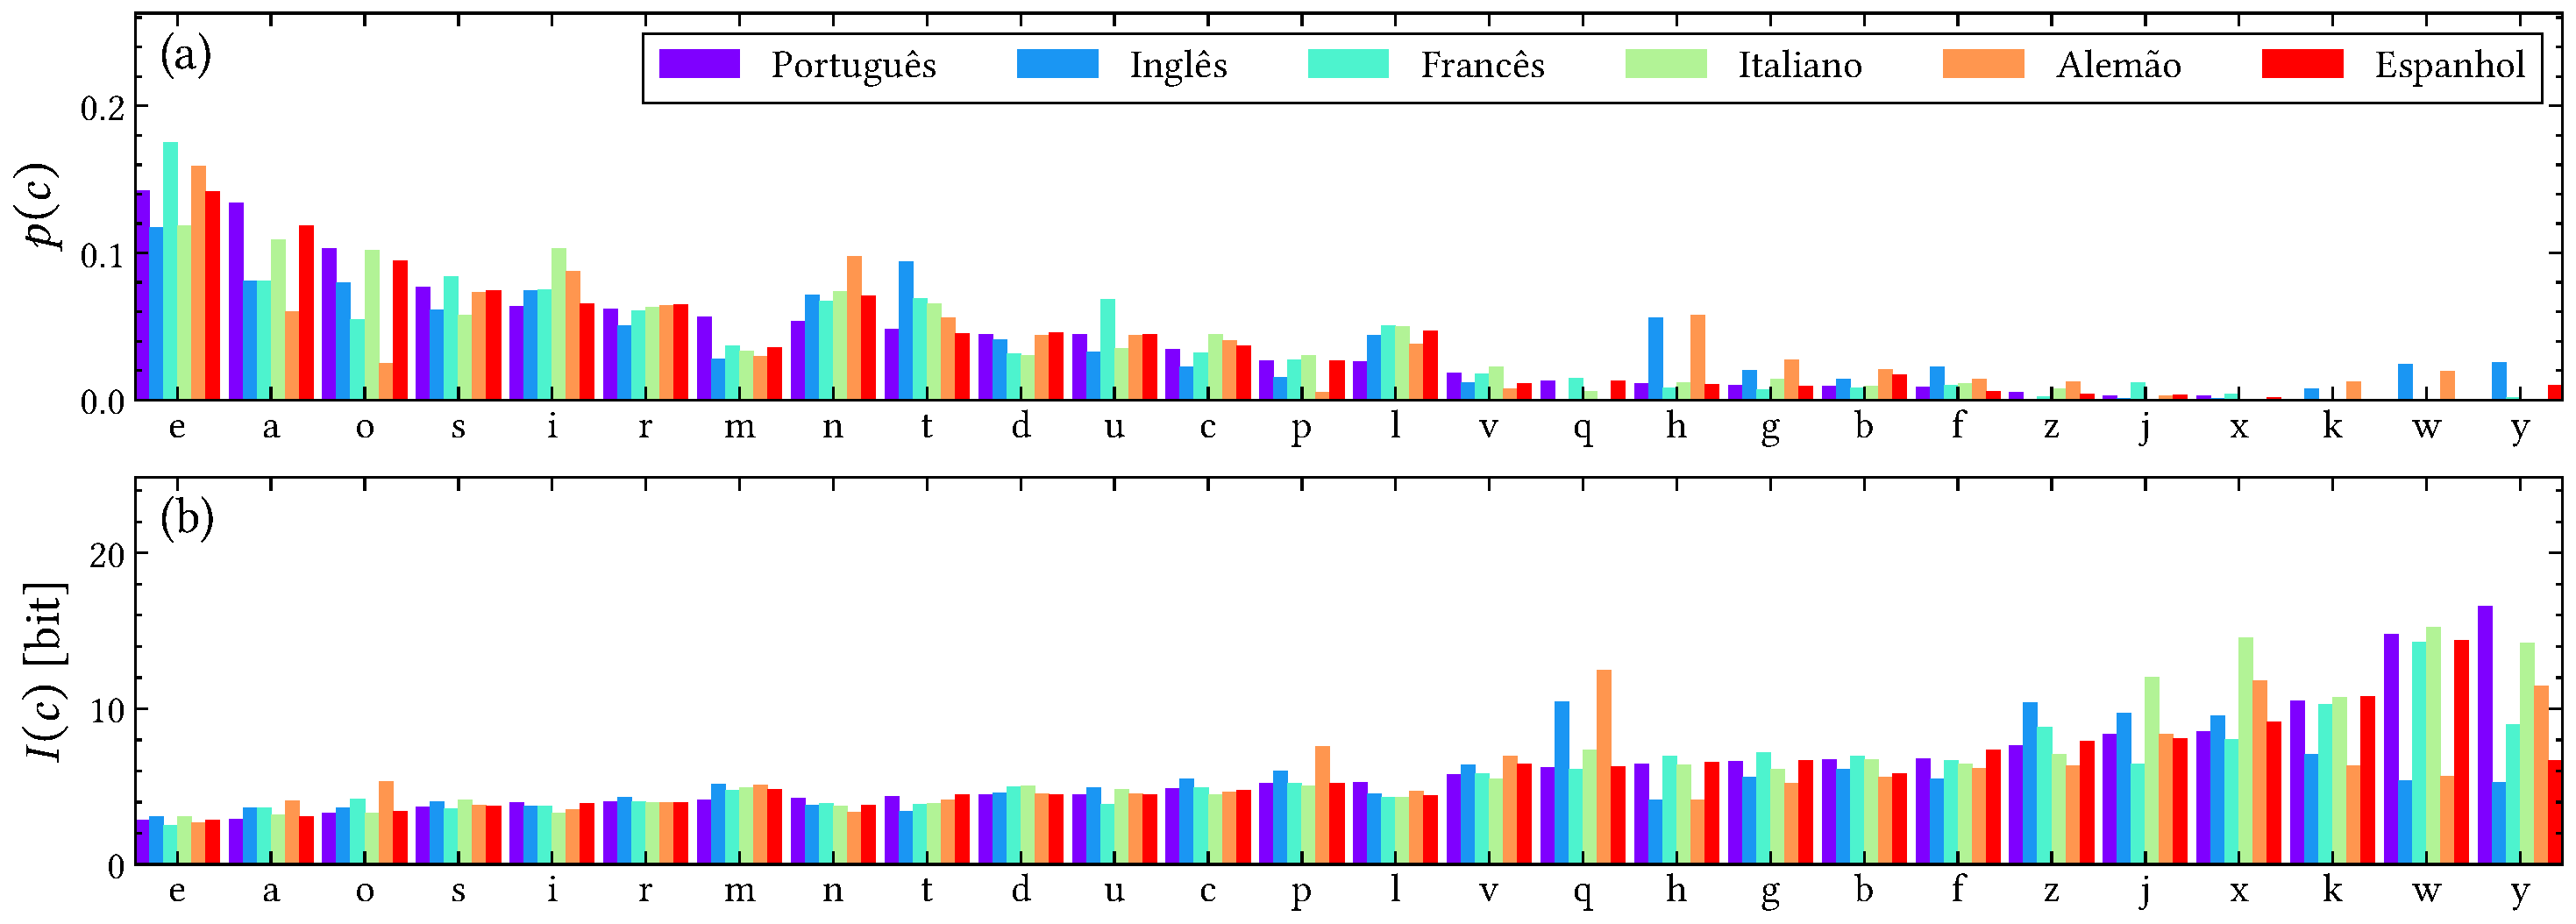
\includegraphics[width=\textwidth]{fig1.pdf}
  \caption{
    (a) Probabilidade de ocorrência de cada letra $p(c)$ para os
    diferentes idiomas escolhidos.
    (b) Informação associada a cada letra $I(c)=-\log_2(p(c))$
    para os idiomas escolhidos.}
  \label{fig:1}
\end{figure*}

A probabilidade de cada letra ocorrer nos idiomas escolhidos
está presente na Fig.~\ref{fig:1}(a), ordenada em ordem
decrescente de probabilidade em Português.
Todos os idiomas escolhidos apresentam probabilidades
similares, com vogais ocorrendo de maneira mais comum
no texto. A exceção à regra é o Alemão, que tem alta
probabilidade de ocorrência de ``r, s'' e ``n''.
Além disso, em todos os idiomas, letras como
``z, j, x, k, w, y'' tem baixa ocorrência. Conforme
mencionado na introdução, essas similaridades indicam
um idioma ancestral em comum.
A quantidade de informação requerida para identificar
cada letra está presente na Fig.~\ref{fig:1}(b);
letras com alta probabilidade necessitam de menos informação para
serem representadas. Por exemplo, a letra ``e'' precisa
de aproximadamente 3 bits para ser representada em Português,
mas a letra ``y'' precisa de quase 18 bits para ser representada;
isso é consequência da baixa probabilidade que a letra ``y'' tem.
De fato, inspecionando o texto, as únicas ocorrências da letra
``y'' são em nomes, e ocorrem nas passagens ``... Hy de Park...'' e
``Byron, Manfredo''. No entanto, no Inglês e Espanhol, a letra
``y'' ocorre com mais frequência, e portanto precisam de menos bits
para serem representadas.

\begin{figure}[!htb]
  \centering
  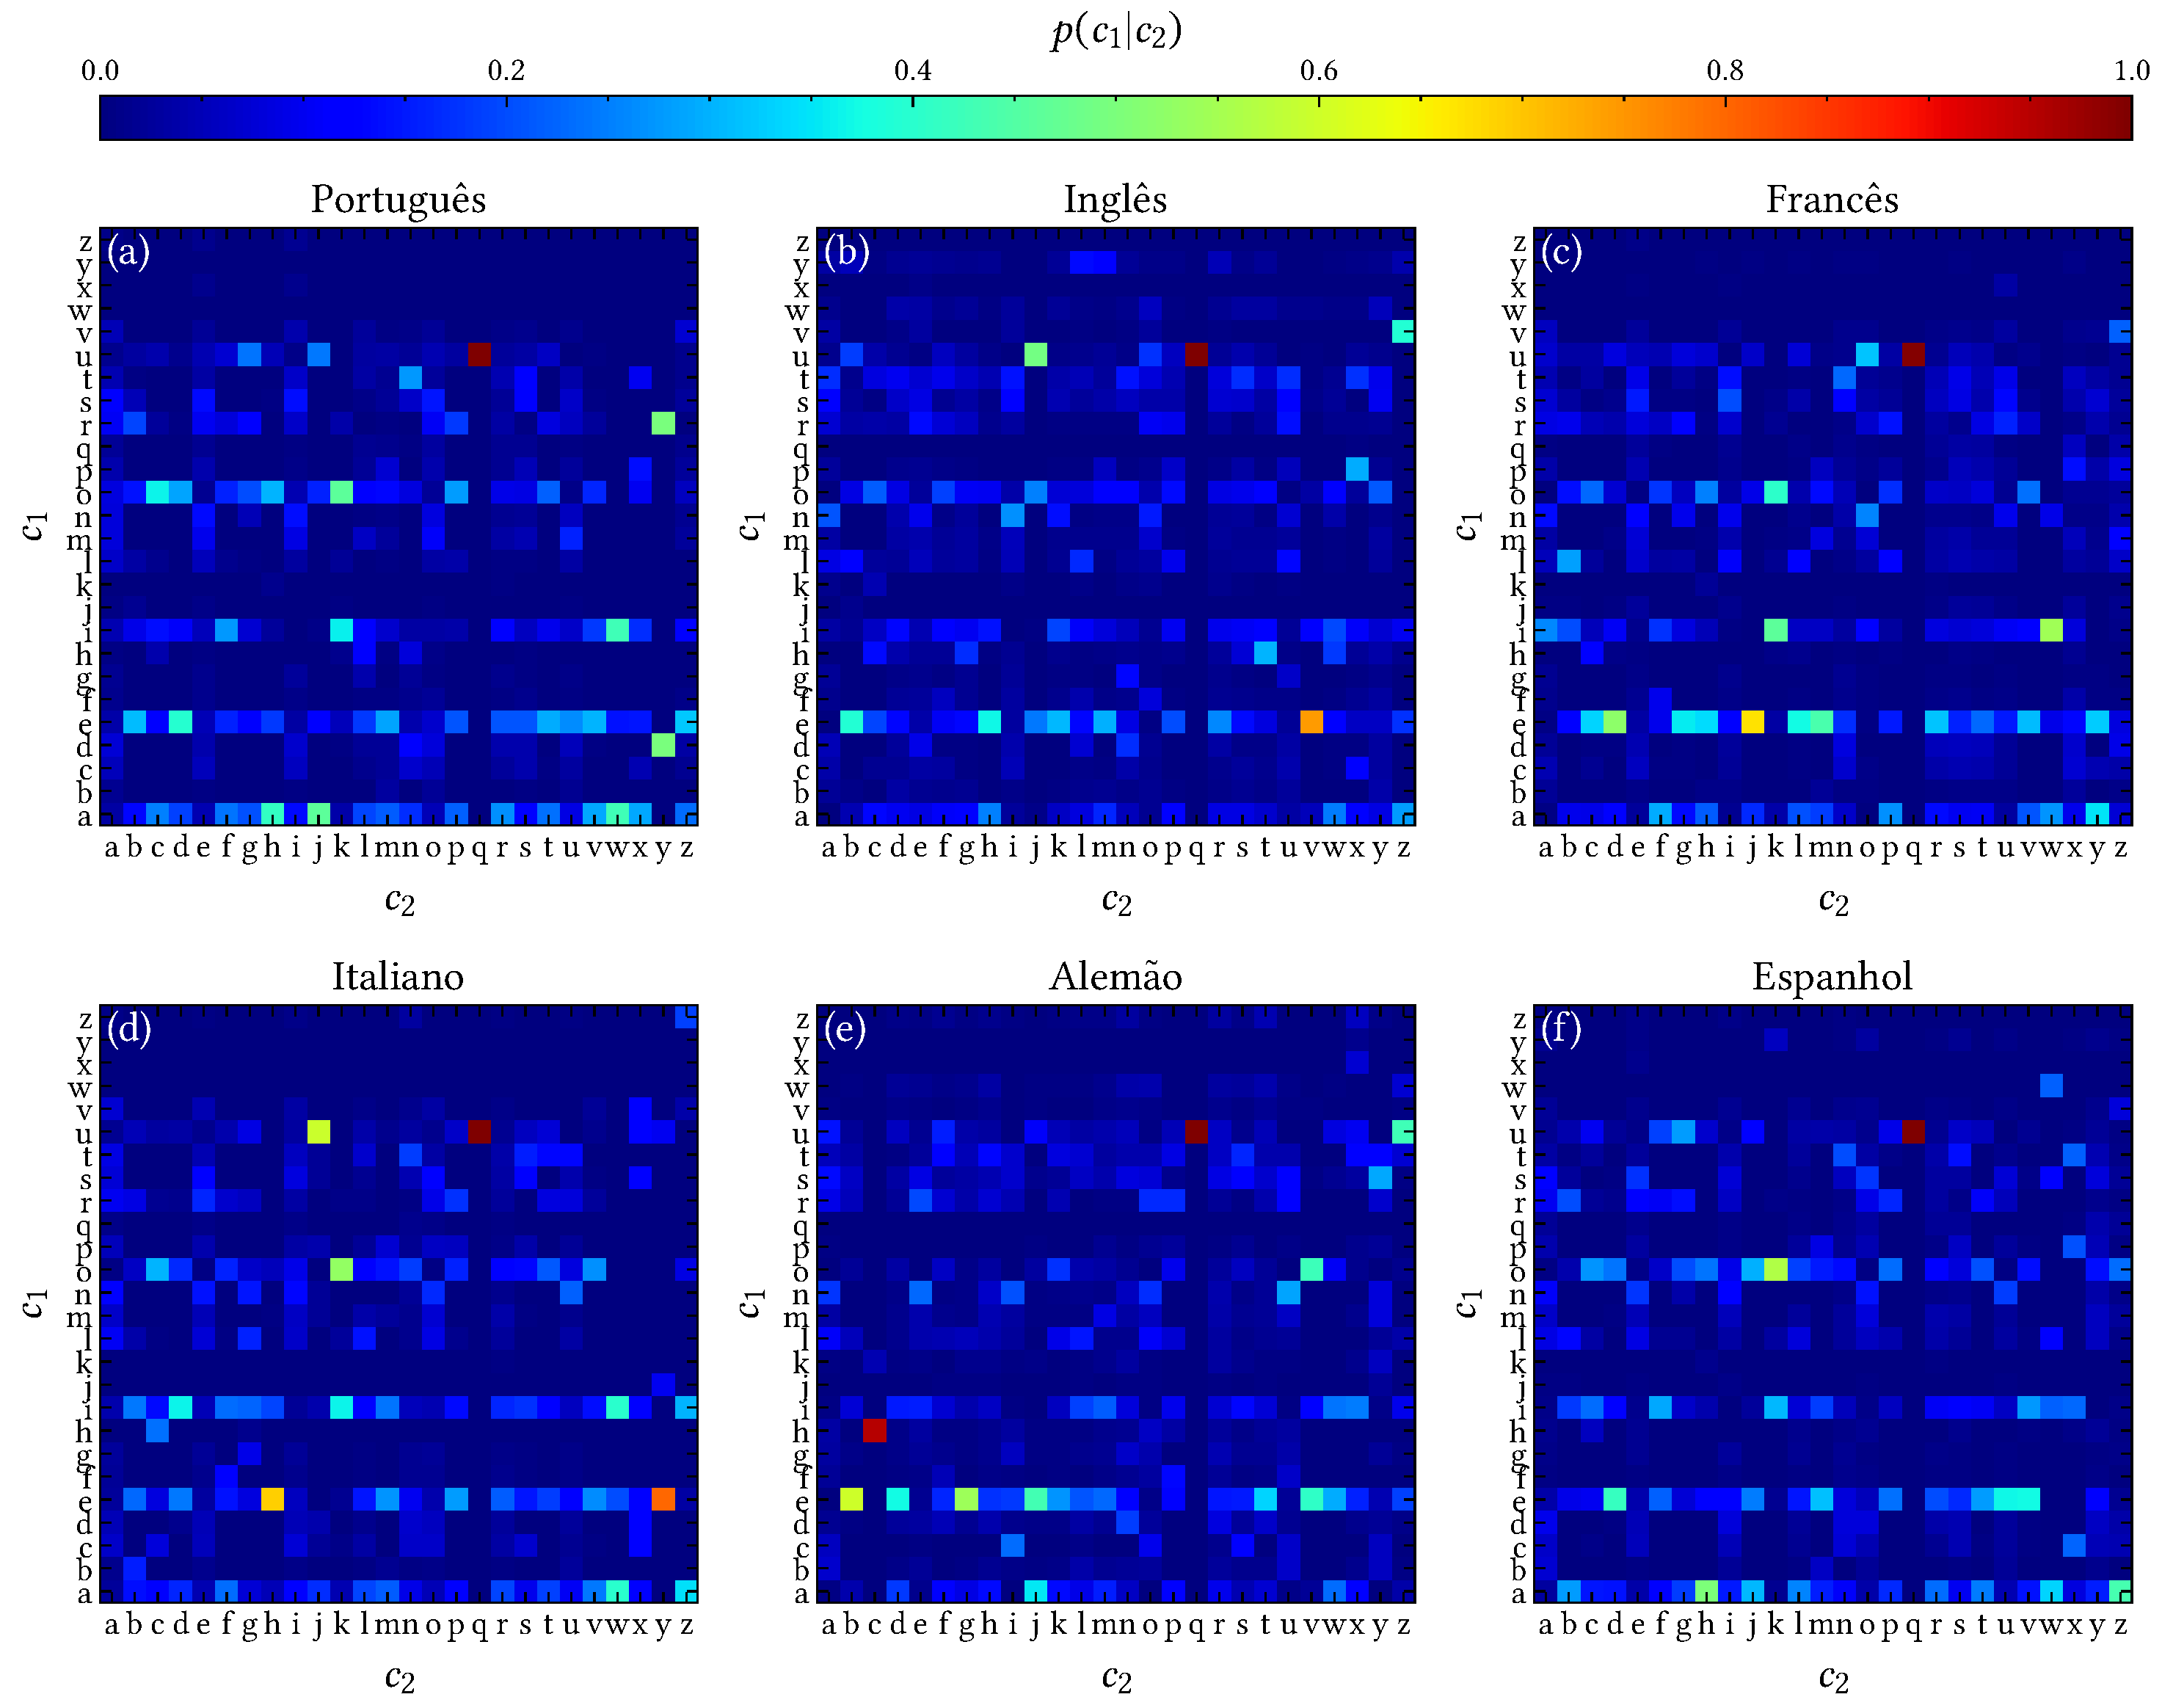
\includegraphics[width=\columnwidth]{fig2.pdf}
  \caption{
    Probabilidade condicional de cada par de letras
    $p(c_1|c_2)$ para os diferentes idiomas escolhidos.
  }
  \label{fig:2}
\end{figure}

Em seguida investigamos a probabilidade
de pares de letras, $p(c_1|c_2)$ para os diferentes
idiomas; o resultado está presente na Fig.~\ref{fig:2}.
Aqui fica evidente que cada idioma tem uma digital que
o identifica univocamente, uma vez que cada idioma
tem $p(c_1|c_2)$ bem diferentes entre si.
Em contraste, existe uma similaridade marcante,
todos os idiomas tem $p(u|q)=1$, ou seja, em todos
idiomas escolhidos depois da letra ``q'' com certeza
virá a letra ``u''. O outro par de letras
que tem $p(c_1|c_2)\approx 1$ é $p(h|c)$ em Alemão,
que tem altíssima probabilidade.

Esse tipo de análise pode ser usada para decifrar
mensagens criptografadas. Conforme mencionado na introdução,
com a informação de que uma mensagem criptografada é
de um dado idioma, é possível montar, após coletadas várias mensagens,
uma análise deste tipo, e usando a digital do respectivo idioma
fazer ``matching'' de pares de letras com o objetivo de determinar
a mensagem original. Essa análise, junto das probabilidades
na Fig.~\ref{fig:1}, podem quase que univocamente e com poucos
erros, determinar a mensagem original.

Agora investigamos a entropia da fonte de cada um
dos idiomas escolhidos, os resultados estão
presentes na tabela~\ref{tab:1} e na Fig.~\ref{fig:3}.
Dentre os idiomas, o Português é aquele que tem menor
entropia da fonte, enquanto Inglês é o com maior
entropia. No caso da entropia de fonte $H(X)$,
os valores oscilam entre $3.979\leq H(X)\leq 4.186$,
um intervalo baixo de variação. Isso indica que
todos os idiomas precisam de aproximadamente o mesmo
tanto de informação média por carácter.
Isso é ainda mais evidente quando investigamos
a entropia condicional $H(X|Y)$, onde o Alemão
tem a menor entropia condicional $H(X|Y)=3.368$, enquanto
o Inglês tem a maior $H(X|Y)=3.608$. No entanto, olhando
pela Fig.~\ref{fig:3}, praticamente todos os idiomas tem
o mesmo valor de $H(X|Y)$, com exceção do Inglês. Novamente
indicando que todos os idiomas precisam de aproximadamente a mesma
informação para representar mensagens.

\begin{figure}[!htb]
  \centering
  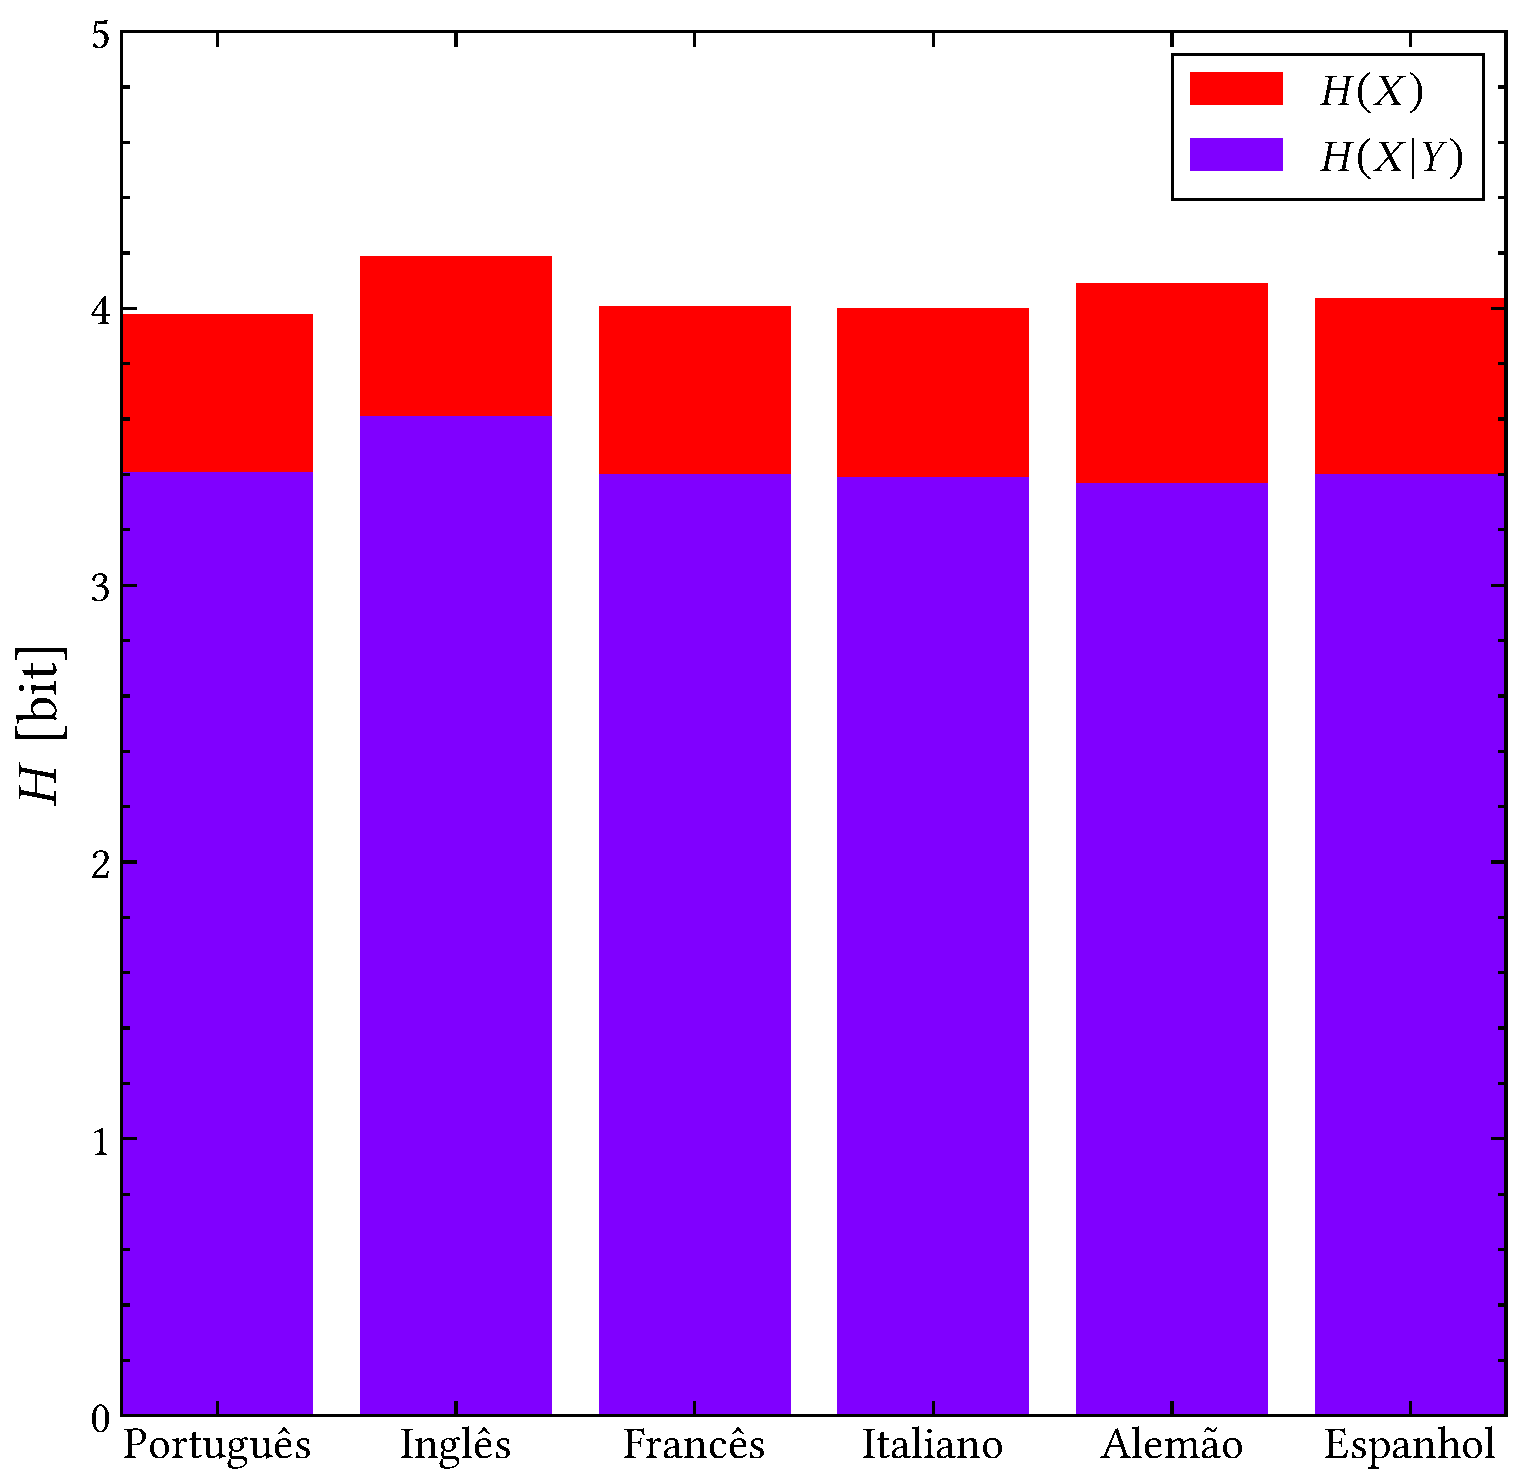
\includegraphics[width=0.8\columnwidth]{fig3.pdf}
  \caption{
    Entropia da fonte $H(X)$ em vermelho,
    e entropia condicional $H(X|Y)$ em roxo,
    para os diferentes idiomas escolhidos. Veja a
    tabela~\ref{tab:1} para os valores numéricos.
  }
  \label{fig:3}
\end{figure}

\begin{table}[!htb]
  \centering
  \begin{tabular}{|c|c|c|}
    \hline
    Idioma & $H(X)$ & $H(X|Y)$ \\
    \hline
    Português & 3.979 & 3.407\\
    \hline
    Inglês & 4.186 & 3.608\\
    \hline
    Francês & 4.008 & 3.398\\
    \hline
    Italiano & 3.999 & 3.389\\
    \hline
    Alemão & 4.091 & 3.368\\
    \hline
    Espanhol & 4.034 & 3.400\\
    \hline
  \end{tabular}
  \caption{Valores das entropias presentes na Fig.~\ref{fig:3}.}
  \label{tab:1}
\end{table}

%\begin{figure}[!htb]
%  \centering
%  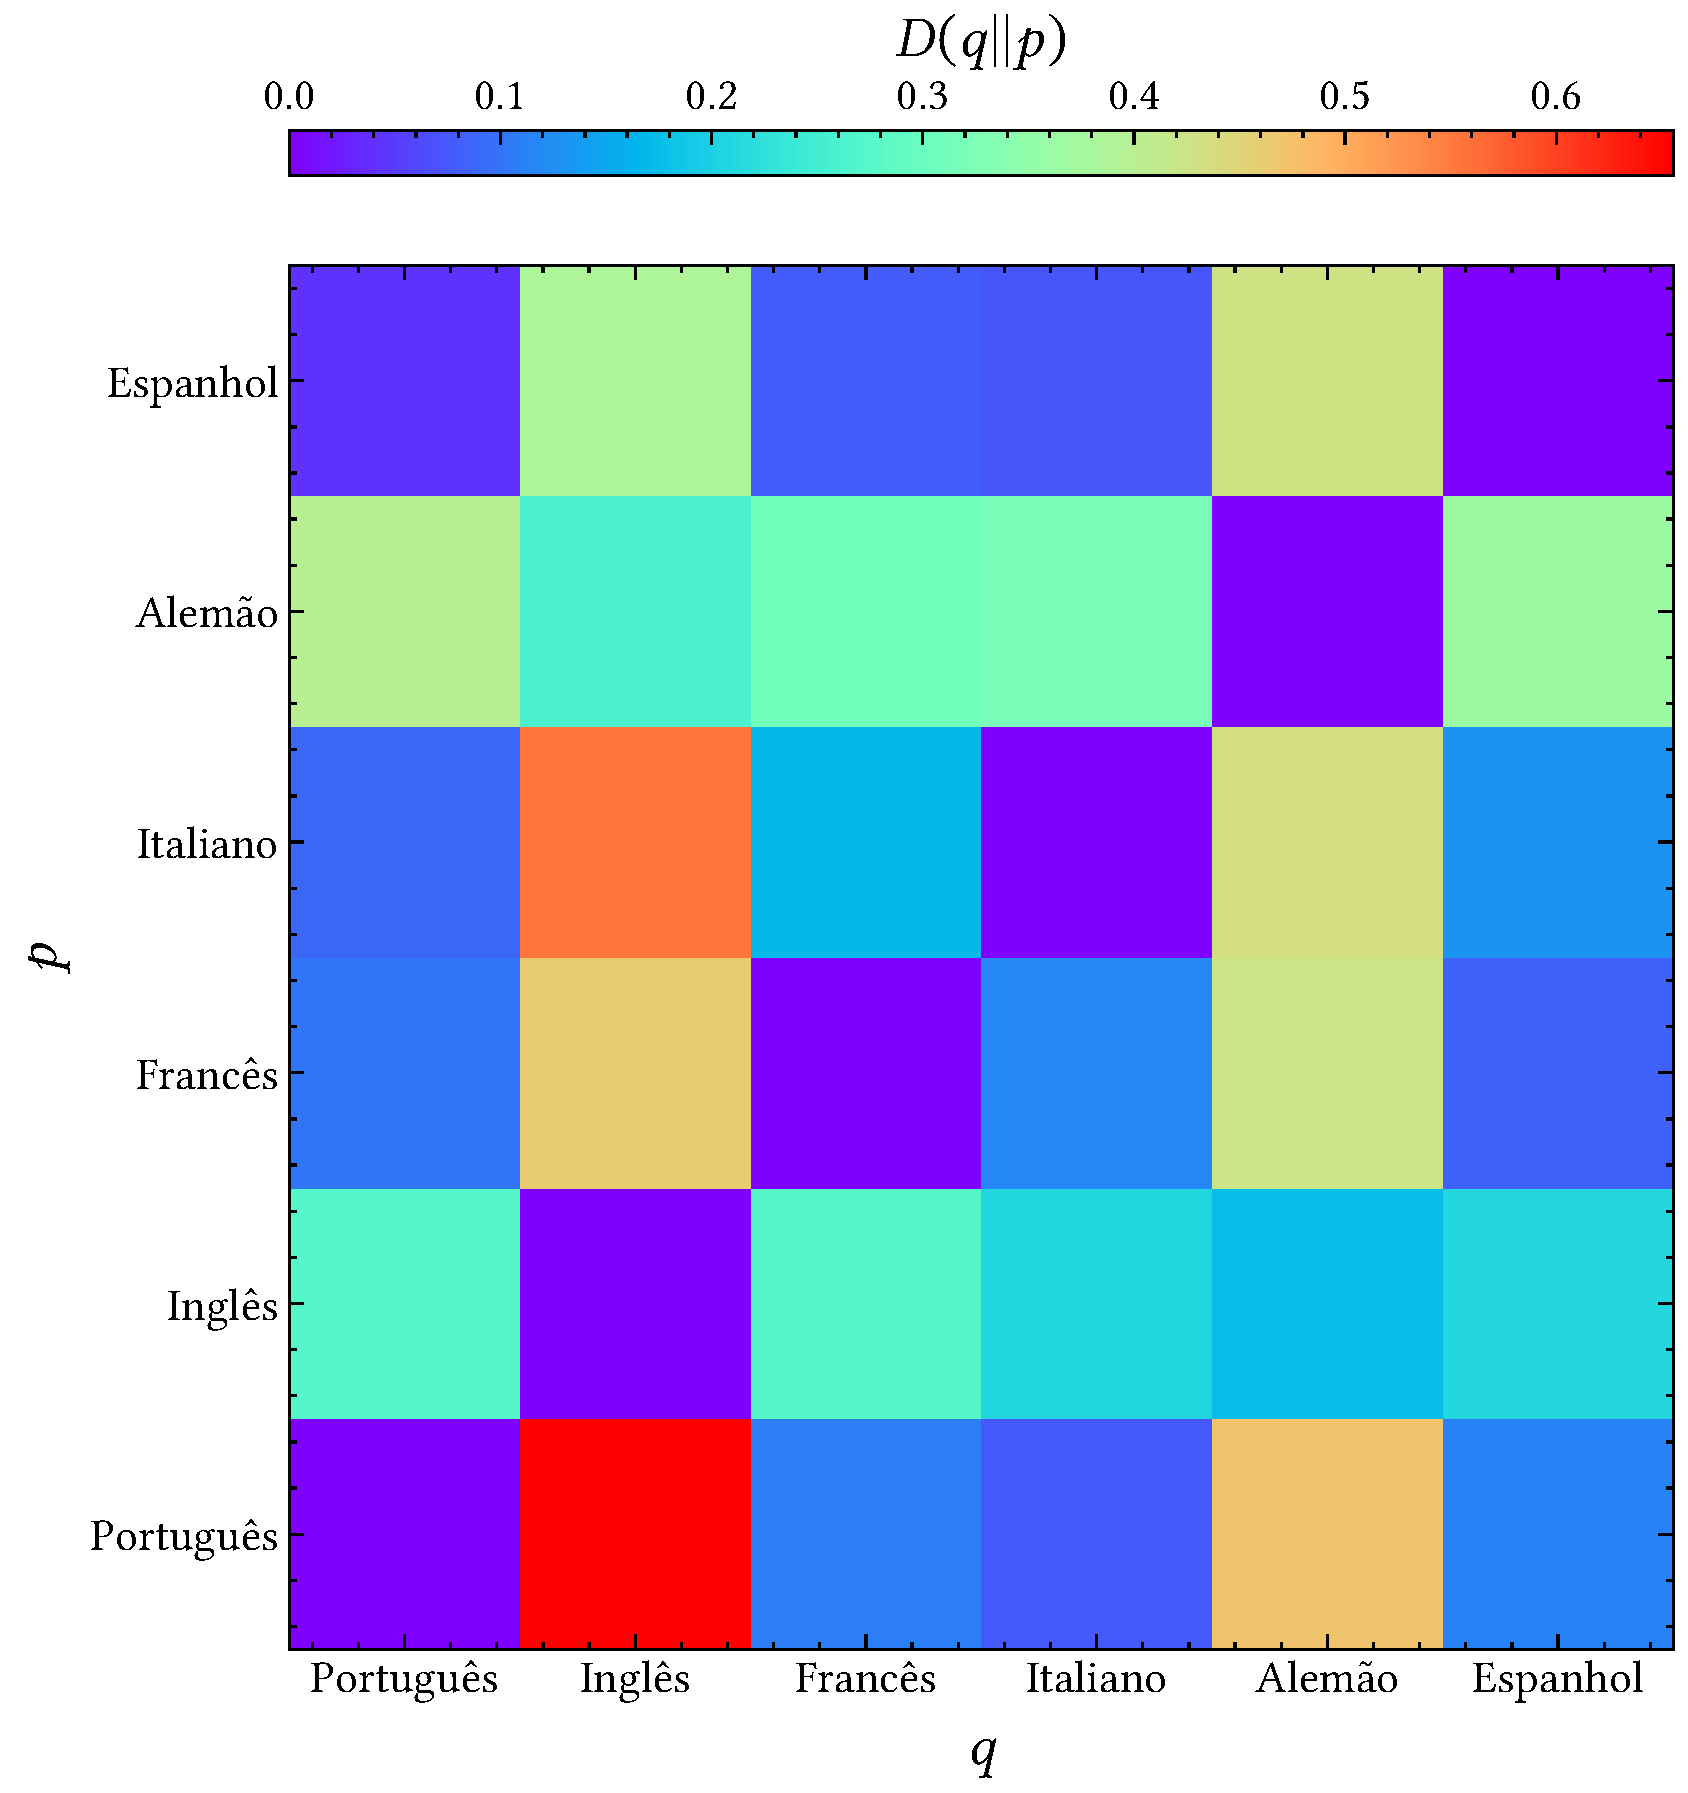
\includegraphics[width=\columnwidth]{fig4.pdf}
%  \caption{
%
%  }
%  \label{fig:4}
%\end{figure}

\begin{figure*}[!htb]
  \centering
  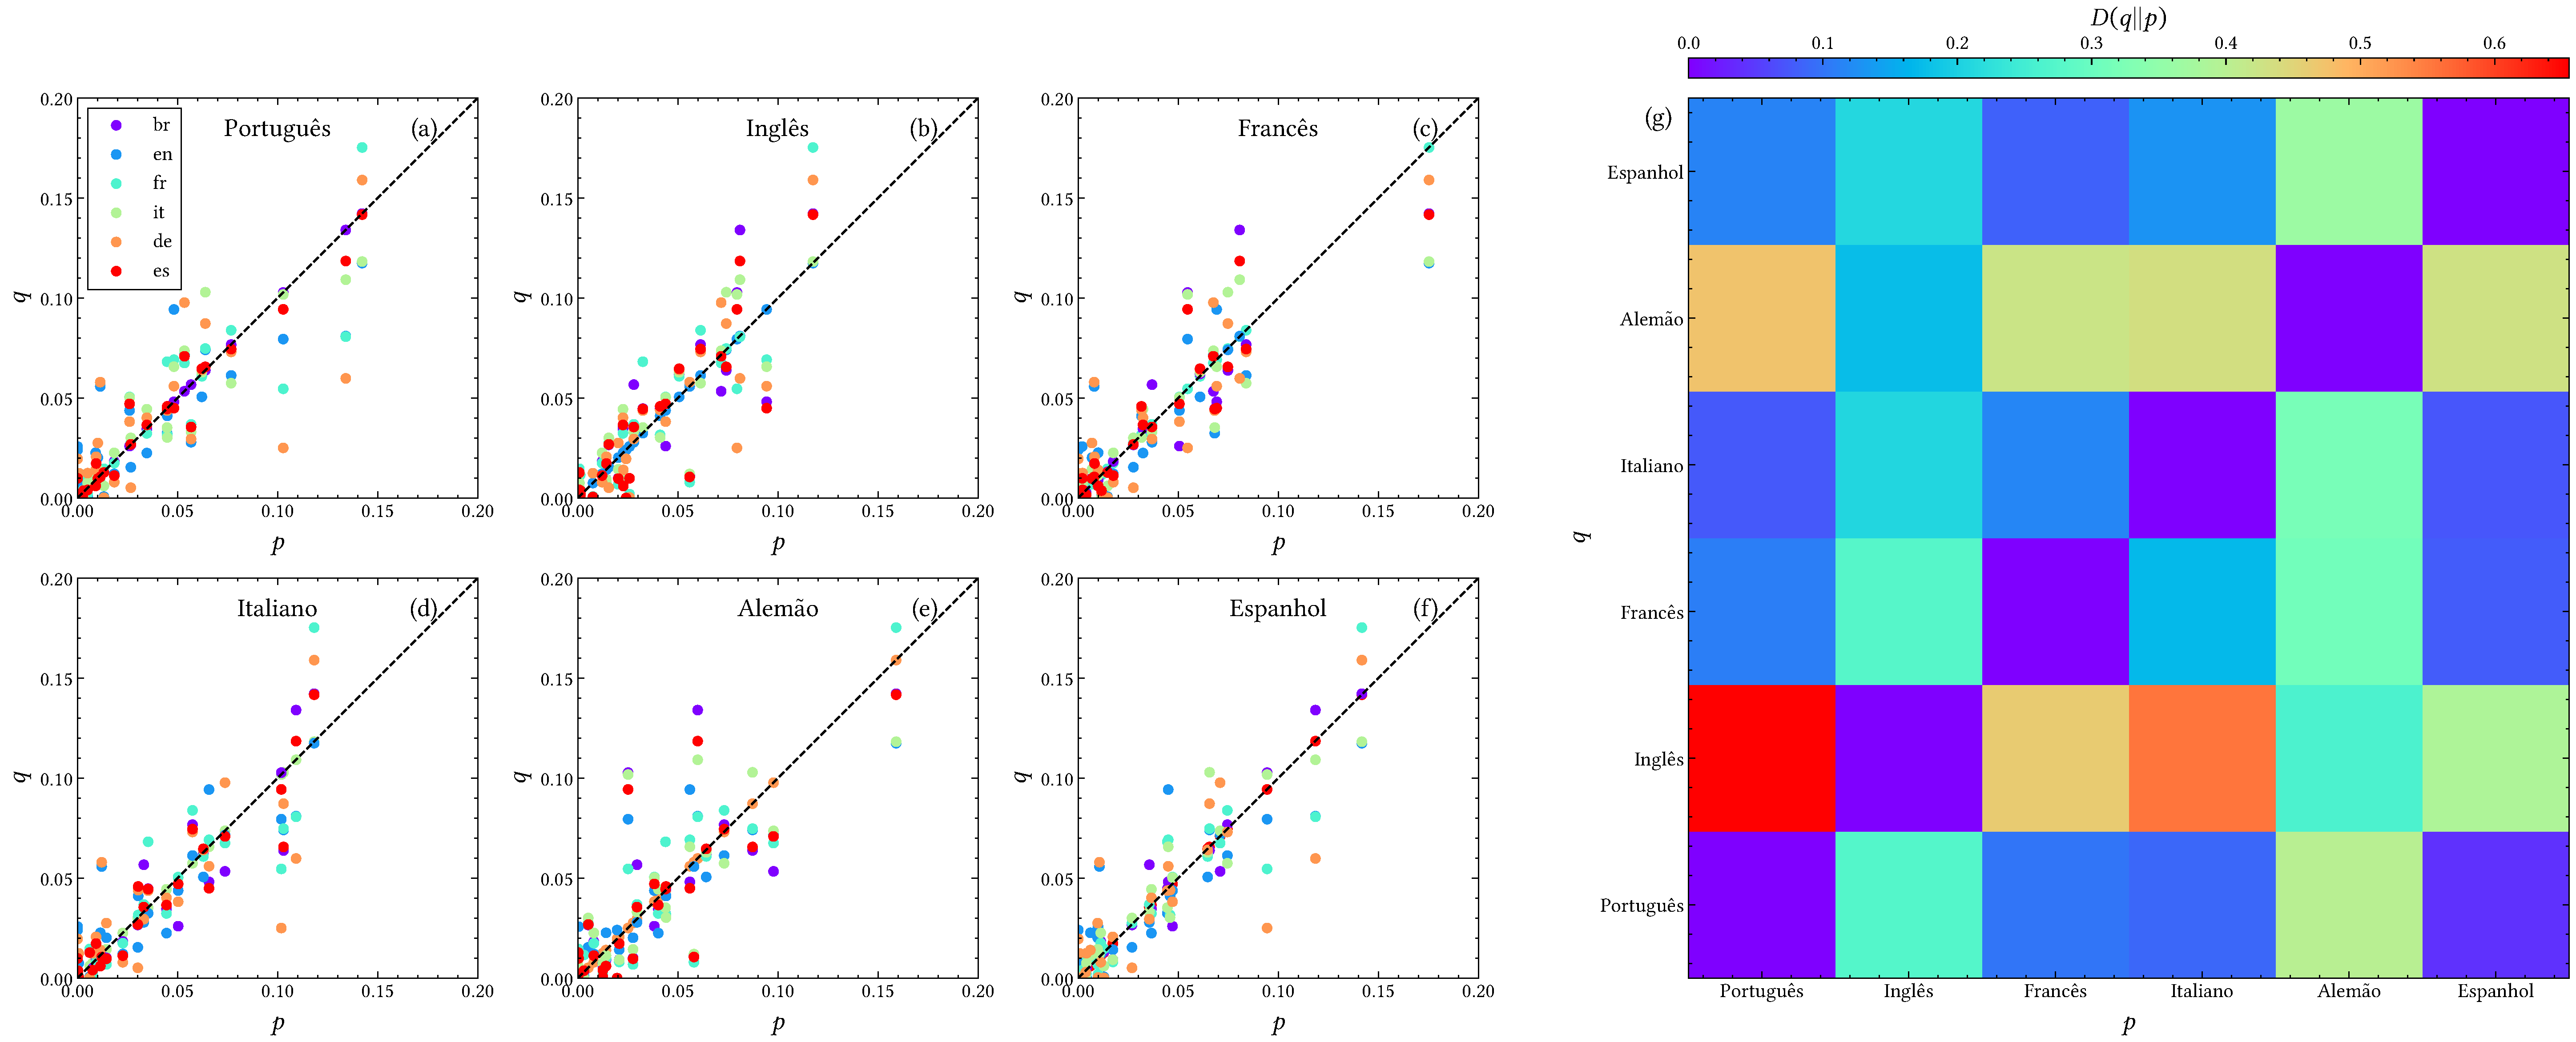
\includegraphics[width=\textwidth]{fig5.pdf}
  \caption{
    (a-f) Correlação entre os caracteres de cada idioma
    com o dos outros idiomas. A linha tracejada corresponde
    à máxima correlação.
    (g) Divergência de Kullback-Leibler $D(q||p)$ entre
    as distribuições de probabilidade associadas
    à cada idioma escolhido.
  }
  \label{fig:5}
\end{figure*}

Por fim investigamos as correlações entre os diferentes idiomas,
e a divergência de Kullback-Leibler, presentes na Fig.~\ref{fig:5}.
Olhando o Português inicialmente, o idioma com maior correlação
é o espanhol, conforme evidenciado pela proximidade
entre a distribuição do Espanhol e do Português na Fig.~\ref{fig:5}(a).
Seguido do Espanhol vem o Italiano e o Francês, com correlações
próximas e distribuições próximas do Português. Depois vem o Inglês com
uma correlação intermediaria, e por último o Alemão, com a menor
correlação com o Português. A medida de correlação é feita usando
a Fig.~\ref{fig:5}(g), e focando na linha referente ao Português.

Embora o Português seja próximo do Inglês segundo
a Fig.~\ref{fig:5}(g), o oposto não é verdade, ou seja,
para o Português o Inglês está próximo, mas para o Inglês
o Português está distante, conforme indicado pelo máximo
valor na Fig.~\ref{fig:5}(g). Diferentemente do Português,
que tinha proximidade com praticamente todos os idiomas escolhidos,
o Inglês é bem distante de dos os idiomas, sendo mais próximo
do Alemão.

O Francês, Italiano e Espanhol apresentam distâncias
relacionados aos outros idiomas bem similares às distâncias
que o Português apresenta. Isso indica que esses idiomas são
próximos entre si e compartilham mais semelhanças do que aparentam,
ao menos do ponto de vista informacional.

Por último, o Alemão apresenta distancias
intermediarias com relação aos outros idiomas.
Embora mais próximo aos outros idiomas do que o
Inglês, o Alemão ainda é bem distante de todos
os outros idiomas, principalmente quando comparado com
Português, Francês, Italiano e Espanhol.

Uma característica importante da Fig.~\ref{fig:5}(g)
é a não simetria de $D(q||p)$, ou seja, $D(q||p)\neq D(p||q)$.
Isso é evidente pelo gráfico e tem como consequência que
a distancia entre uma distribuição e outra depende de
quem é usado como base. Por exemplo, para o Português
o Inglês está relativamente próximo, mas para o Inglês
o Português está o mais distante possível.

Uma outra métrica que poderia ser utilizada para determinar a
correlação é a métrica $R^2$ comumente utilizada para
determinar o quão bom foi o resultado de uma regressão linear.
Nesse caso, a ``regressão linear'' é a reta $y=x$, representando
a máxima correlação. No entanto, esperamos que essa medida
nos de aproximadamente a mesma informação que a Fig.~\ref{fig:5}(g)
já fornece.

\section{Conclusão}

Usando o livro ``Memórias do Subsolo'' de Fiódor Dostoiévski,
investigamos as características que diferentes idiomas
apresentam do ponto de vista informacional.
Vimos que dentre os idiomas escolhidos, embora
sejam visivelmente diferentes, apresentam similaridades do ponto
de vista informacional. Uma delas é a frequência de vogais, que
é predominante em todos os idiomas com exceção do Alemão.

Usando $p(c_1|c_2)$ em conjunto com $p(c)$
observamos que é possível criar uma digital para um certo idioma,
possibilitando determinar o idioma de uma mensagem suficientemente
longa, além da possibilidade de determinar univocamente possíveis
criptografias feitas, principalmente as mais simples, tipo a cifra de Caesar. Aqui foi observado que todos os idiomas tem $p(u|q)=1$, ou seja,
depois de um ``q'' com certeza virá um ``u'', indicando que um idioma
ancestral entre todos esses idiomas existe, e muito possivelmente
tinha essa característica com relação ao ``u'' e ``q''.

Do ponto de vista de entropia da fonte, e entropia condicional,
não existe uma diferença muito grande com relação aos idiomas, o que
indica que os idiomas escolhidos requerem aproximadamente o
mesmo tanto de informação para codificar mensagens. Isso é
especialmente verdade para a entropia condicional, que pode ser
considerada aproximadamente constante.

Por fim investigamos correlações entre os idiomas através
da divergência de Kullback-Leibler, e observamos que
o Português, Francês, Italiano e Espanhol estão próximos
dos outros idiomas escolhidos, enquanto que o Inglês
e o Alemão estão mais distantes. A baixa distância
dos idiomas mencionados possivelmente se deve à um idioma
ancestral comum entre eles, que por diferentes fenômenos,
deu origem aos idiomas atuais.

\bibliography{bibliography}

\end{document}
